\chapter{Serviços}

\section{Achados e perdidos}

    A UFBA, em si, não possui um serviço voltado para objetos achados e perdidos na universidade.
    
    Entretanto, um grupo de alunos da univerdade criou uma página, no Facebook, na qual as pessoas compatilham objetos que perderam ou que acharam.
    
        
    \subsubsection{Achados e Perdidos - UFBA}
    
    ``Perdeu ou encontrou algo nas dependências da universidade? Então, deixe o espírito da honestidade falar mais alto e compartilhe conosco! Mandem as informações por inbox. ;)''
    
    \begin{figure}[!htb]
        \centering
        
\includegraphics[width=0.5\textwidth]{achadoseperdidos}
    \end{figure}

\section{Assistência Jurídica}

        Subdividi-se em Assistência e Assessoria.
        
    \begin{itemize}
        \item Assistência: acompanhamento de demandas processuais individuais em matérias de Direito, com exceção das áreas Penal e Trabalhista. 
        \item Assessoria: na perspectiva da educação popular, trabalho com Movimentos Sociais de Luta pela Terra e Luta por Moradia, tais como, respectivamente, o CETA – Movimento Estadual de Trabalhadores Assentados, Acampados e Quilombolas - e o MSTB – Movimento dos Sem-Teto da Bahia.
    \end{itemize}
    
    \subsubsection {Dias da Semana e Horário de Atendimento:}
        2ª e 6ª das 14h00 às 17h00 \\
        3ª e 4ª das 14h00 às 17h00 e das 18h30 às 20h30 \\
        5ª das 18h30 às 20h30
 
    \subsubsection {Telefone de Atendimento ao Cidadão:}
        (71) 3283-9050

    \subsubsection {Email de Atendimento ao Cidadão:}
        sajubahia@gmail.com
        
    \subsubsection{Maiores informações:}
        http://www.sajubahia.blogspot.com
   
    \subsubsection{Sistema de Sugestões e Reclamações:}
        Telefone: (71) 3283-9050 \\
        Email: sajubahia@gmail.com

    \subsubsection{Endereço de Atendimento:}
        Faculdade de Direito da UFBA \\
        R. da Paz, s/n, Graça, Salvador-BA
        
    \subsubsection{Requisitos, Documentos e Informações necessárias para acessar o serviço:}   
        \begin{enumerate}
            \item  Requisitos: Impossibilidade de arcar, individualmente, com despesas processuais
            \item Documentos: Cédula de Idenditade, CPF, Comprovante de Residência, Comprovante de Renda
            \item Informações Necessárias: relato da problemática que dará, ou não, inicio a um processo
        \end{enumerate}

\begin{wrapfigure}{r}{0.4\textwidth}
        \centering
        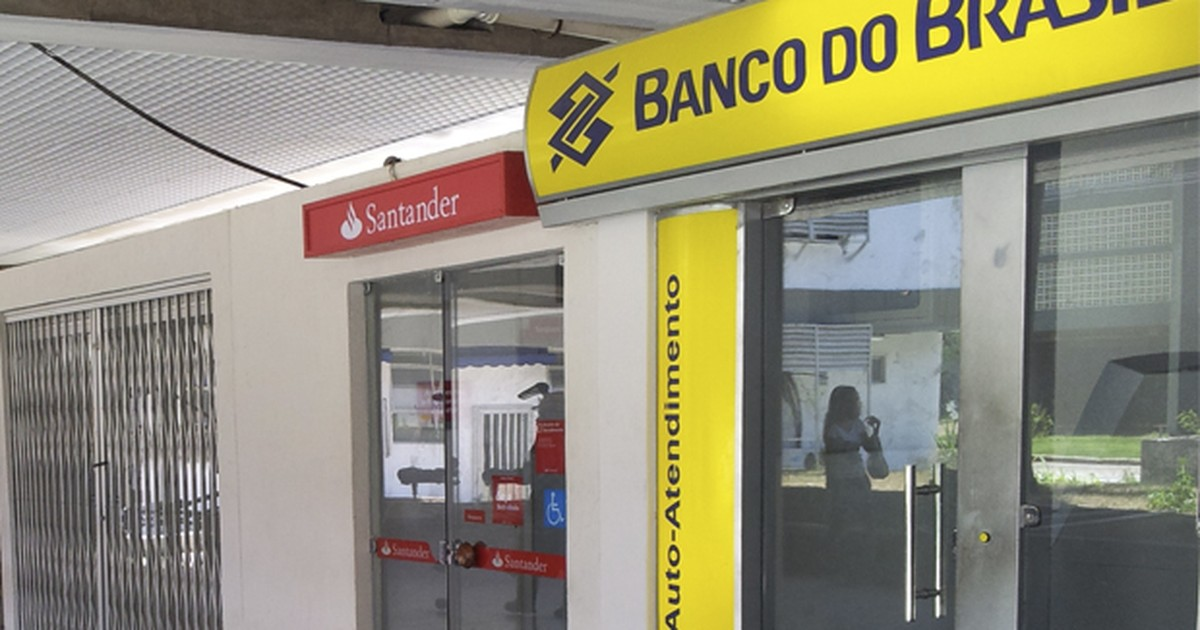
\includegraphics[width=0.39\textwidth]{bancos}
    \end{wrapfigure}
\section{Bancos}
     O estudante pode contar com as unidades de auto atendimento dos bancos Santander e Banco do Brasil que há ao lado do PROAE.
     
     Próximo ao Campus da Ondina, há algumas agências de banco que podem ser utilizadas pelos estudantes da UFBA, 10 minutos a pé, a partir da entrada principal do campus Ondina. São elas: Agência Santander, Banco do Brasil, Banco Itaú e Caixa Econômica Federal.
      
\section{BURMC}

    \begin{wrapfigure}{r}{0.4\textwidth}
        \centering
        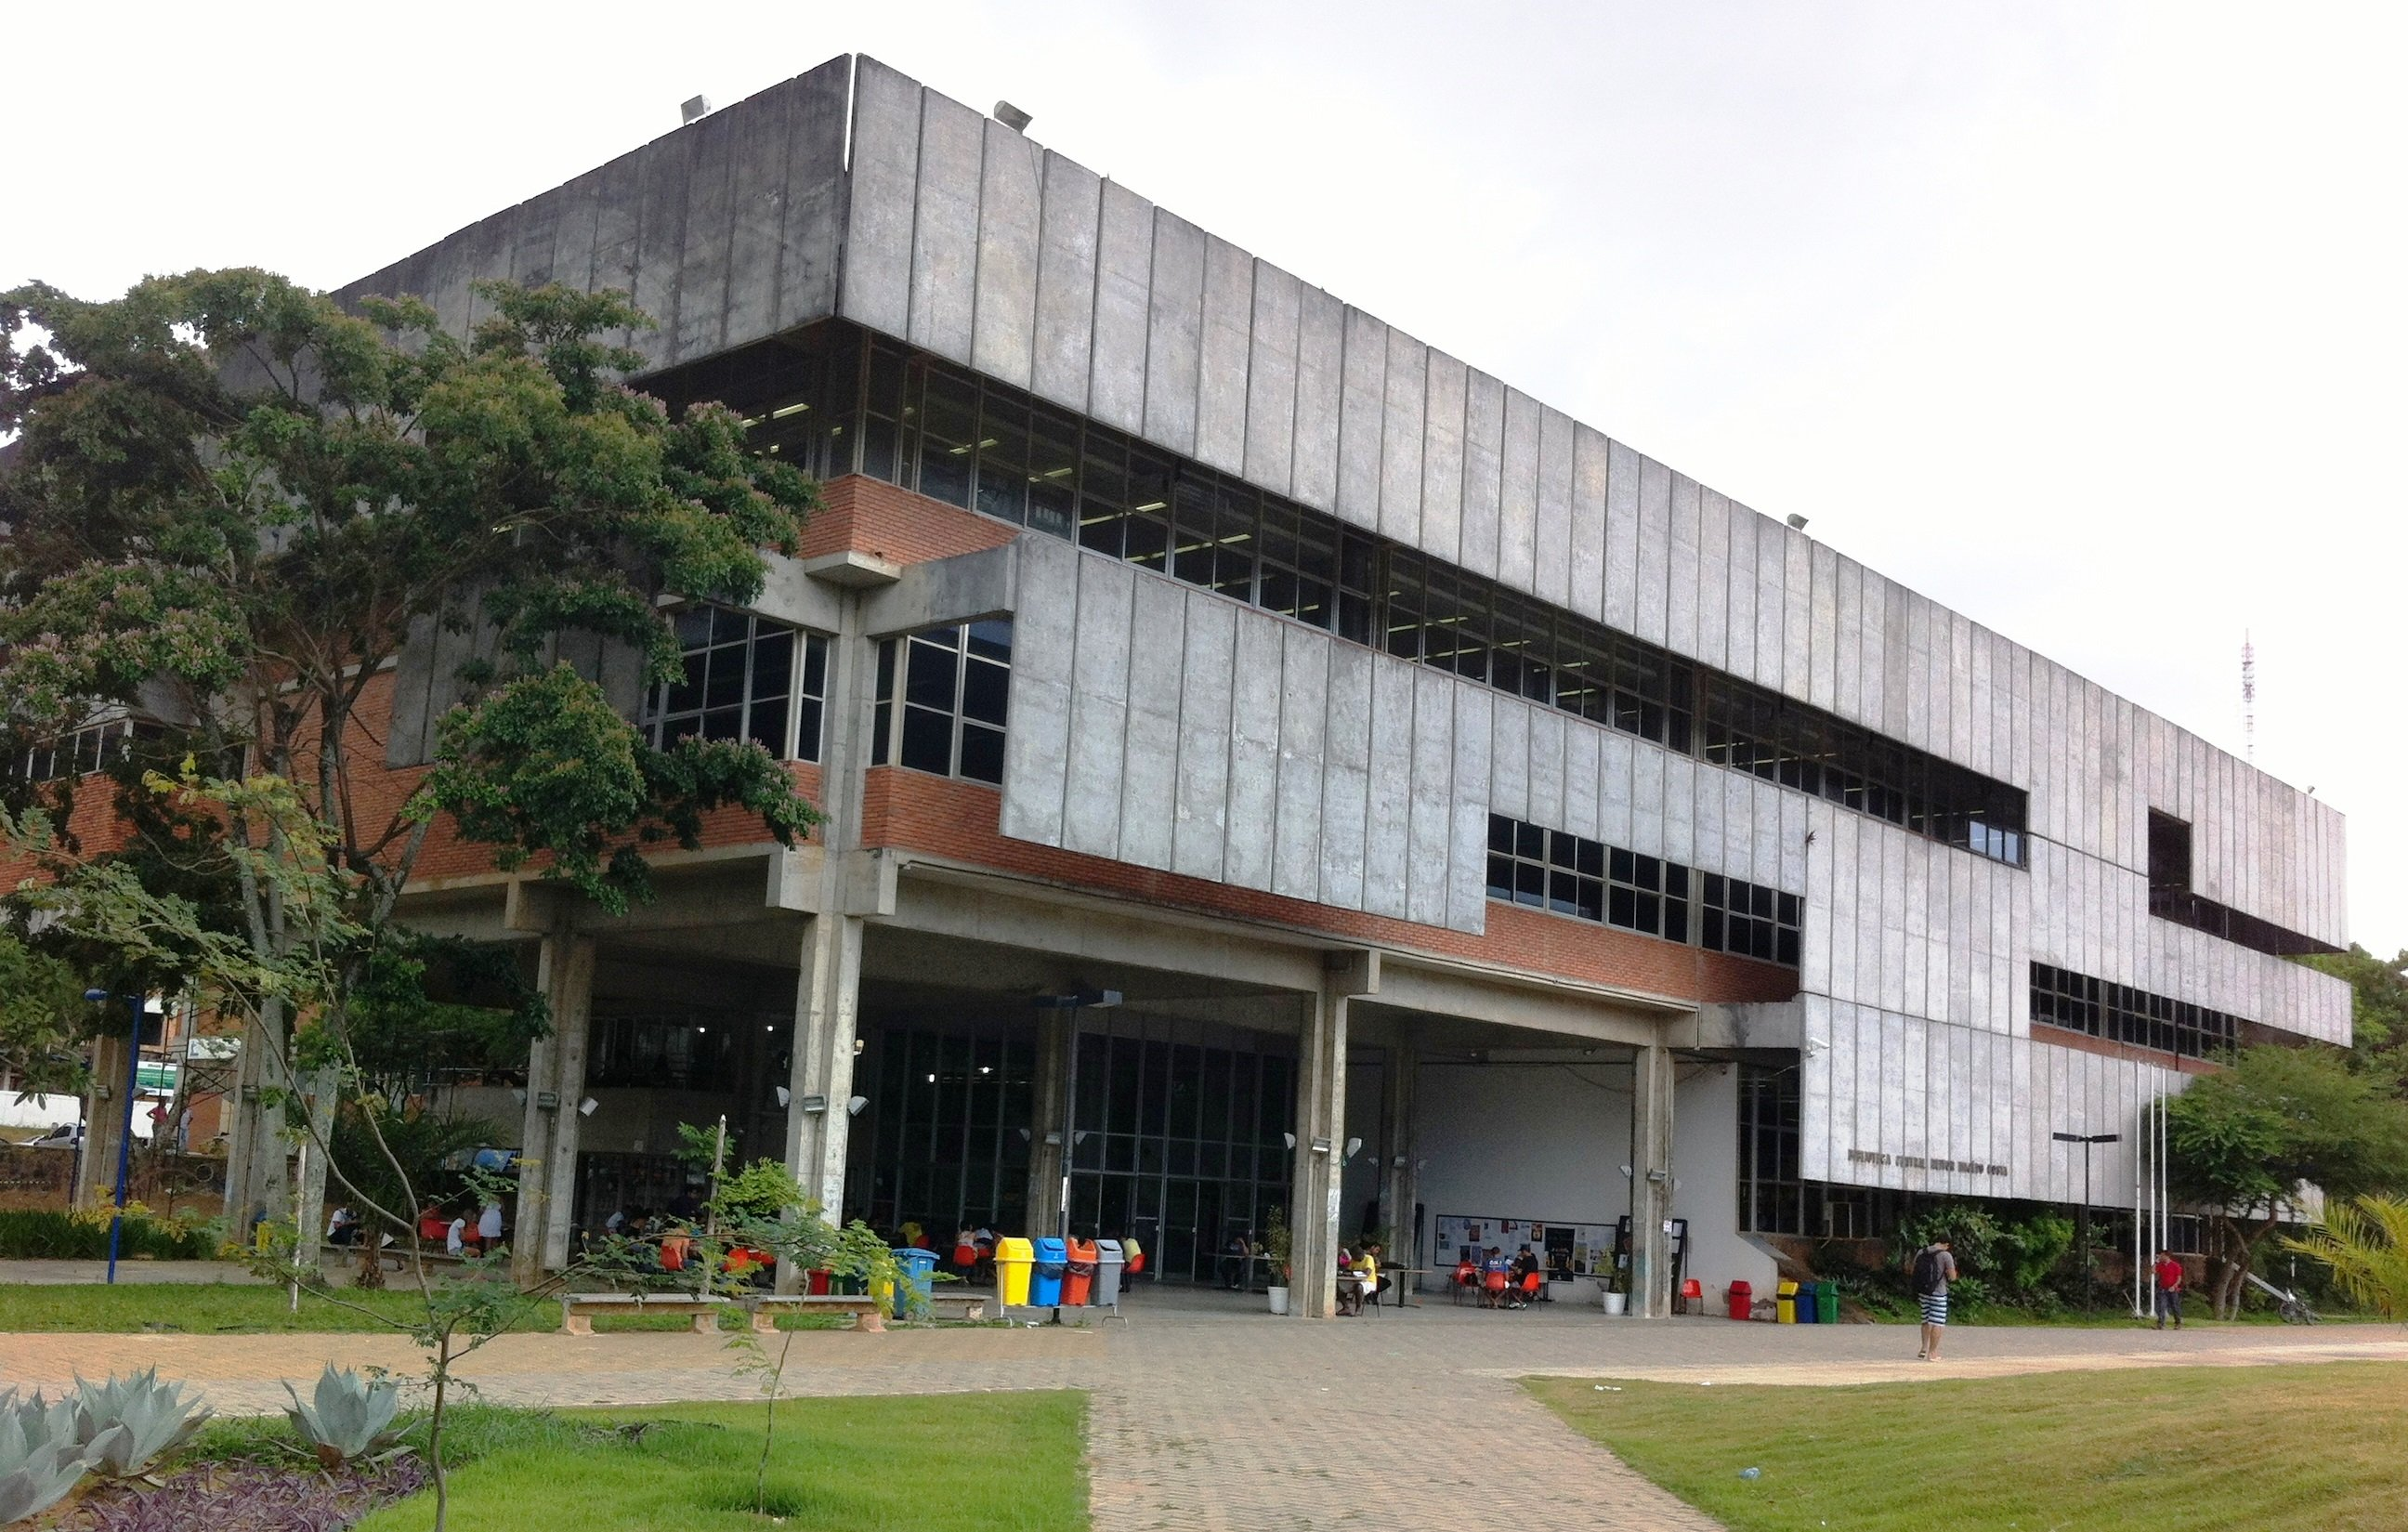
\includegraphics[width=0.39\textwidth]{biblioteca}
    \end{wrapfigure}

    
    Ou Biblioteca Universitária Reitor Macedo Costa,  é uma das diversas bibliotecas que faze parte do SIB- Sistema de Bibliotecas da UFBA- atende através do emprésctimo de livros (Comunidade Interna), consultas  (serviço personalizado) e orientação à normalização de trabalhos científicos e técnicos. O estudante UFBA pode fazer uso de determinado livro por um período limitado apresentando número de matrícula e a senha escolhida no momento do cadastro.

        \subsubsection{Telefone:}
            (71) 3283-6060 
        
        \subsubsection{Endereço:}
            (Campus Universitário de Ondina) Rua Barão de Jeremoabo s/n,  Salvador, BA.
            CEP.: 40170-290
            
        \subsubsection{Dias de Funcionamento:}
            Segunda a Sábado
            
        \subsubsection{Requisitos:}
            \begin{enumerate}
                \item  Estudante: Comprovante de matricula
                \item Servidores: Matricula SIAPE
                \item Comunidade externa: Apresentação de um documento com foto
            \end{enumerate}
        \subsubsection{Email}
             bcdir@ufba.br
        \subsubsection{Mais informações:}
            http://www.sibi.ufba.br
    
\section{Conectividade}

\begin{wrapfigure}{r}{0.35\textwidth}
    \centering
    
\includegraphics[width=0.34\textwidth]{logo-new}
\end{wrapfigure}

O serviço de Conectividadade à Rede UFBA é prestado pela Superintendência de Tecnologia da Informação da UFBA (STI-UFBA), e tem como objetivo prover o compartilhamento de recursos e acesso à Internet para os usuários da comunidade acadêmica e visitantes.

Computadores, impressoras, scanners, notebooks, smartphones,entre outros, podem integrar a Rede UFBA através da tecnolgia de rede cabeada ou sem fio (wi-fi).

    \subsubsection{Rede Cabeada}
        \begin{itemize}
            \item Quem tem acesso? \\
            Funcionários da UFBA (docentes e técnicos administrativos), terceirizados, alunos bolsistas (graduação e pós-graduação). \\
            
            \item Como?\\
            Por meio de um usuário e senha devidamente configurados pelo responsável de T.I. da unidade 
        \end{itemize}
        
    \subsubsection{Rede Wi-Fi}
        
        A rede sem fio é dividida em: \\
        \begin{itemize}
            \item UFBA-Academica: rede segura para o acesso de docentes, técnicos-administrativos, terceirizados, alunos bolsistas. \\
            
            \item UFBA-Administrativa: rede segura para o acesso de docentes, técnicos-administrativos, terceirizados, alunos bolsistas. \\
            
            \item UFBA-Visitantes: rede aberta ao uso de todos.
        \end{itemize}
        
    \subsubsection{Como acessar o serviço?}
        Realize a abertura de chamado, que pode ocorrer:
        
        \begin{itemize}
            \item Online: https://webdesk.ufba.br/MRcgi/MRentrancePage.pl \\
            
            \item Por meio dos canais de Comunicação da Central de Serviços:\\
            Telefone: (71) 3283-6100 das 7h00 às 22h00 \\
            E-mail: helpdesk@ufba.br
        \end{itemize}

\section{Correios}

        Hoje em dia, a gama de prestação de serviços e o leque de produtos que os Correios oferecem, ultrapassam as fronteiras das remessas de correspondências, cartas e outros itens.
        Por isso, pensando no melhor tratamento e entrega de correspondências, encomendas e documentos em qualquer ponto do território nacional, a UFBA disponibiliza em sua estrutura uma Agência dos Correios.
        
        \subsubsection{Telefone:}
            (71) 3237-0005
            
        \subsubsection{Endereço:}
            Av. Adhemar de Barros, s/n, Ondina, Salvador - BA 
            CEP: 40170-110
            
        \subsubsection{Horário de Funcionamento:}
            De 2ª a 6ª, das 09:00 às 17:00

        \subsubsection{Mais informações:}
            www.correios.com.br
            
\section{EDUFBA}
    \begin{wrapfigure}{r}{0.25\textwidth}
        \centering
        
\includegraphics[width=0.20\textwidth]{edufba}
    \end{wrapfigure}
   
    Editora Gráfica Universitária, publica originais, desde que aprovados pelo seu conselho editorial, de produção ciêntifíca universitária, como teses de doutorado e dissertações de mestrado. Dispõe de três livrarias nas quais comercializa não só sua produção, como as de outras intituições e editoras privadas, elas são: \\
    
        
    \begin{itemize}
        \item EDUFBA Livraria 1    
            \subsubsection{Endereço:} 
            Biblioteca Universitária de Saúde Professor Álvaro Rubim de Pinho
            
            Rua Basílio da Gama, s/n
            
            (ao lado da Escola de Enfermagem)
            
            Campus do Canela
            
            40110-909 Salvador-BA
            \subsubsection{Telefone e FAX:}
             (71) 3283-7075 \\
             
        \item EDUFBA Livraria 2
        
           \subsubsection{Endereço:}
           Rua Barão de Jeremoabo, s/n
            
            (Biblioteca Reitor Macedo Costa)

            Campus de Ondina

            40170-115 
            
            Salvador-BA
            
            \subsubsection{Telefone e FAX:}
            (71) 3283-6165 \\
            
        \item EDUFBA Livraria 3 CEAO
        
            \subsubsection{Endereço:}
            Praça Inocêncio Galvão, 42

            Largo Dois de Julho

            40060-180 
            
            Salvador-BA
            
            \subsubsection{Telefone e FAX:}
            (71) 3322-6742
            
        \end{itemize}
        
    \subsubsection{Email:}
        edufba@ufba.br
        
    \subsubsection{Mais informações:}  
        http://www.edufba.ufba.br
        
\section{Fotocópias}
    Há serviços de copiadoras e xerox oferecidos ao redor do IHAC, PAF 3, estes localizam-se:

    \subsubsection{Letras, Facom}
        Funciona das 8h às 19h
        
    \subsubsection{Biologia}
        Funciona das 8h às 20h
        
    \subsubsection{Matemática}
        Funciona das 7h30 às 21h
        
    \subsubsection{}
    Os valores a seguir são comuns a todos os estabelecimentos: 
    Até dez (10) cópias 10 centavos e, a partir de 11 cópias, 9 centavos
    
    \begin{remark} 
    A ação Xerox na Ufba, ou Rinoufba, é uma comunidade com propósitos sustentáveis de reaproveitamento da xerox na UFBA, pela qual se pode vender, doar, adquirir e comprar Xeroquiados usados e semi-novos.
    \subsubsection{Mais informações:}
    https://www.facebook.com/acao.xerox/
    \end{remark}
    
\section{Laboratórios}
    \subsection{LACTFAR}
    
    O LACTFAR desenvolve atividades de extensão juntamente com as atividades de ensino e pesquisa.
    
    \begin{wrapfigure}{r}{0.5\textwidth}
        \centering 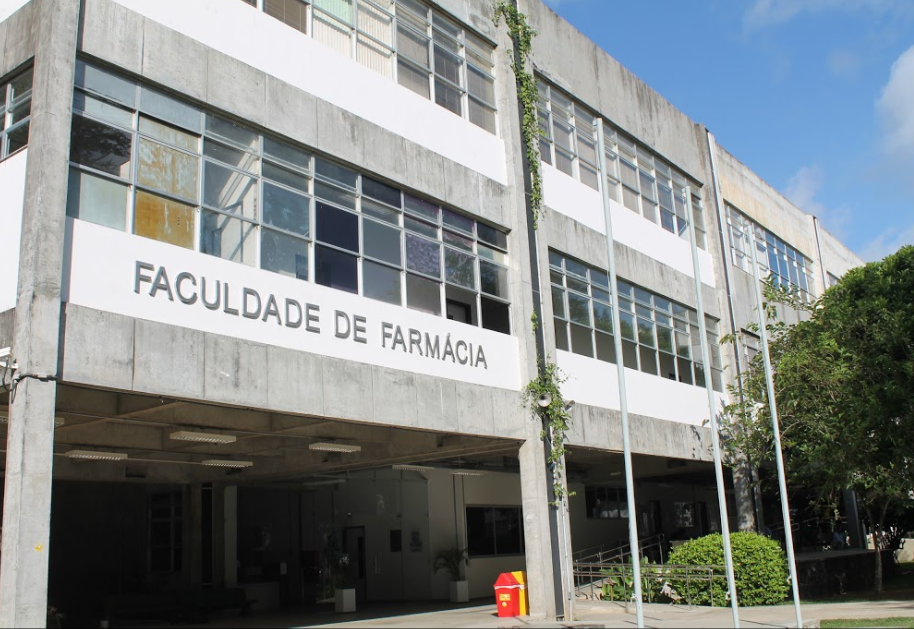
\includegraphics[width=0.49\textwidth]{lactfar}
    \end{wrapfigure}

    São atendidos, em médica, cerca de 160 pacientes por dia, encaminhados pelo SUS, por meio do convênio entre a Prefeitura Municipal de Salvador e a UFBA.
    
    Por meio dessa parceira, são realizados exames de baixa, média e alta complexidade, nas áreas de bioquímica, biologia molecular, imunologia das doenças auto-imunes e das doenças infecciosas, hematologia, parasitologia e toxicologia. 
    
    Além disso, este laboratório funciona como um Laboratório Escola, onde os alunos da graduação e da pós-graduação desenvolvem atividades.
    
    Ainda, o Laboratório realiza diagnósticos de doenças endêmicas e não endêmicas, que são de relevância para a Saúde Pública do Estado da Bahia.

    
    \subsubsection {Dias da Semana e Horário de Atendimento:}
        De 2ª a 6ª: 
        \begin{itemize}
            \item entrega de senha a partir da 06h30
            \item atendimento das 07h00 às 10h00
        \end{itemize}
 
    \subsubsection {Telefone de Atendimento ao Cidadão:}
        (71) 3283-6974 \\
        (71) 3283-6948
        
    \subsubsection {Email de Atendimento ao Cidadão:}
        recepcao.lactfar@gmail.com
   
    \subsubsection{Sistema de Sugestões e Reclamações:}
        Telefone: (71) 3283-7044 \\
        Email: ouvidoria@ufba.br

    \subsubsection{Endereço de Atendimento:}
        Faculdade de Farmácia da UFBA, campus Ondina \\
        R. Barão de Jeremoabo, s/n, Ondina, Salvador-BA
        
    \subsubsection{Requisitos, Documentos e Informações necessárias para acessar o serviço:}   
        Requisição médica do SUS, Cartão SUS, Comprovante de Residência e Documento de Identificação com Foto
    

    \subsection{Laboratório de Imunologia}
    
     
        Vinculado ao Instituto de Ciências da Saúde da UFBA, o laboratório
    realiza exames de imunodiagnóstico e imonodosagem, assim como desenvolve projetos de pesquisa na área da imunologia veterinária, padronização de ensaios sorológicos para doenças humanas e de animais domésticos. 
    
        Além disso, tem como contribuir para a formação de pessoas
    voltadas para as práticas e atividades acadêmicas, assim como prestar atendimento à comunidade por meio da realização de cerca de 300.000 testes anuais, entre ensaios sorológicos, dosagens de hormônios e de marcadores tumorais, bem como imunofenotipagens de hemopatias malignas. 

    \subsubsection {Dias da Semana e Horário de Atendimento:}
        De 2ª a 6ª das 6h00 às 11h30 e das 13h00 às 17h00
 
    \subsubsection {Telefone de Atendimento ao Cidadão:}
        (71) 3235-9682 \\
        (71) 3245-5971
        
    \subsubsection {Email de Atendimento ao Cidadão:}
        labimuno@labimuno.org.br
        
    \subsubsection{Maiores informações:}
        http://www.labimuno.org.br
   
    \subsubsection{Sistema de Sugestões e Reclamações:}
        Telefone: (71) 3283-8179 \\
        Email: ouvidoria@hupes.ufba.br

    \subsubsection{Endereço de Atendimento:}
        Instituto de Ciências da Saúde, térreo \\
        Av. Reitor Miguel Calmon, s/n, Vale do Canela, Salvador-BA
        
    \subsubsection{Requisitos, Documentos e Informações necessárias para acessar o serviço:}   
        Guias do SUS corretamente preenchidas, assinadas e carimbadas pelo médico, assim como autorizadas pelo SUS. Documento de Identificação com foto e cartão SUS.

\section{Redes Sociais}
    Nas redes sociais, o estudante encontrará:
    
        \subsubsection{Grupo da UFBA}
        O grupo público e geral de discussões e avisos da UFBA, no Facebook, criado por alunos da universidade

        \subsubsection{Grupo do Curso de Ciência da Computação da UFBA}
        O grupo fechado de discussões e avisos, no Facebook, voltados aos estudantes do Bacharelado de Ciência da Computação da UFBA
        
        \subsubsection{Página DCC UFBA(@dcc1968)}
        A página do Departamento de Ciência da Computação da UFBA (DCC-UFBA).
        
        \subsubsection{Página InfoJr UFBA (@infojrnews)} 
        A página da Empresa Júnior de Informática (InfoJr)
        

\section{Saúde Animal}
    \subsection{Hospital de Medicina Veterinária}
            
            \begin{wrapfigure}{r}{0.5\textwidth}
        \centering
 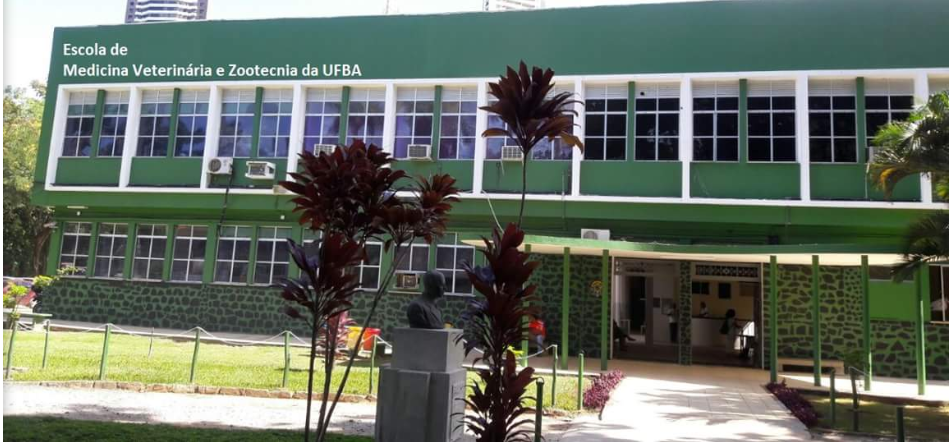
\includegraphics[width = 0.49\textwidth]{medvet}
    \end{wrapfigure}
    
        O Hospital de Medicina Veterinária da UFBA possui a importante missão de prestar assistência médica à animais de pequeno médio e grande porte da comunidade acadêmica e da população em geral. 
        
        Além disso, tem como objetivo formar pessoas voltadas para as práticas e atividades acadêmicas, além de oferecer atendimento à pesquisa docente. 
        
       
        
    Dentre os serviços prestados estão:
        
        \begin{itemize}
            \item Atendimento clínico 
	        \item Atendimento cirúrgico
	        \item Vacinação de cães e gatos
	        \item Atendimento clínico à campo para animais de produção
	        \item Diagnósticos por imagem (Ultrassonografia, Raio-X, Eletro e Ecocardiograma)	
	        \item Diagnósticos e Serviços Laboratoriais \\
	        (Lab. Análises Clínicas, Lab. Viroses, Lab. Bacterioses, Lab. Reprodução, Lab. Parasitoses, Lab. Anatomia Patologia, Lab. Tuberculose e Lab. Micoses)
        \end{itemize}
        
        \subsubsection{Dias da Semana e Horário de Funcionamento:}
            De 2ª a 6ª das 7h às 17h
    
        \subsubsection {Telefone de Atendimento ao Cidadão:}
            (71) 3235-8770 \\
            (71) 3283-7044

        \subsubsection{Email de Atendimento ao Cidadão:}
            hospmed@ufba.br
    
        \subsubsection{Sistema de Sugestões e Reclamações:}
            Telefone: (71) 3283-7044 \\
            Email: ouvidoria@ufba.br

        \subsubsection{Endereço de Atendimento:}
            Av. Ademar de Barros, Ondina,Salvador – BA \\
            CEP: 40170-010

        \subsubsection{Requisitos, documentos e informações necessárias para acessar o serviço:}
            Documento de Identificação com Foto e CPF do dono do animal
\section{Saúde Humana}
    \subsection{Complexo HUPES}
    
     \begin{wrapfigure}{r}{0.4\textwidth}
        \centering
        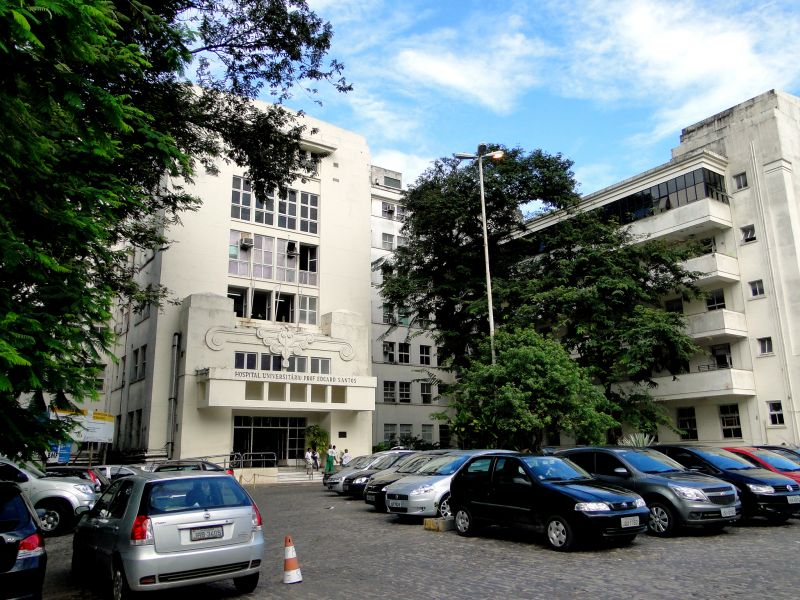
\includegraphics[width=0.39\textwidth]{hupes}
    \end{wrapfigure}
    
    É constituído pelo Hospital Professor Edgard Santos (Hospital das Clínicas), pelo Centro Pediátrico Professor Hosannah de Oliveira (CPPHO) e pelo Ambulatório Professor Magalhães Neto (AMN)
    
    \subsubsection{Dias da Semana e Horário de Funcionamento:}
            \begin{itemize}
                \item Internação: 24 horas
                
                \item Exames e setores administrativos:
                De 2ª a 6ª, das 07h às 16h ou das 07h às 19h
            \end{itemize}
    
    \subsubsection {Telefone de Atendimento ao Cidadão:}
            (71) 3283-8000

    \subsubsection{Email de Atendimento ao Cidadão:}
            superintendenciahupes@gmail.com
    
    \subsubsection{Sistema de Sugestões e Reclamações:}
            Email: ouvidoria@hupes.ufba.br \\ Telefone: (71) 3283-8179

    \subsubsection{Endereço de Atendimento:}
            Rua Augusto Viana, s/n, Canela, Salvador - BA

    \subsubsection{Requisitos, documentos e informações necessárias para acessar o serviço:}
            Requisição do médico, cartão HC (Hospital das Clínicas) e cartão SUS.
    
    \subsection{Centro Docente Assistencial de Fonodiaulogia}
    
     Clinica-escola onde realizam-se atendimento à comunidade nas áreas de fonoterapia e audiologia.

    \subsubsection{Para marcação de consultas e demais informações:}
            De 2ª a 6ª, das 8h às 12h e das 12h às 17h, pelo telefone (71)3283-8887 ou (71)98726-4079 ou via presencial

    \subsubsection{Email de Atendimento ao Cidadão:}
            cedaf@ufba.br
    
    \subsubsection{Sistema de Sugestões e Reclamações:}
            Email: cedaf@ufba.br \\ Telefone: (71) 3283-7044

    \subsubsection{Endereço de Atendimento:}
            Instituto de Ciências da Saúde (ICS)/UFBA, no primeiro andar. Av. Reitor Miguel Calmon, s/n, Vale da Canela, Salvador-BA
            
    \subsubsection{Exames oferecidos:}
            Audiometria, Imitanciometria e BERA (PEATE)

    \begin{remark}
            Já para consulta fonoaudiológica para terapia/avaliação (queixas na voz, linguagem oral e escrita,
            motricidade orofacial ex:
            mastigação, respirador oral, interposição de língua, etc), realizamos cadastro em
            lista de espera (dados completos do paciente, telefone, queixa), tanto por telefone como presencial. Para
            consulta não é obrigatório encaminhamento (pode ser demanda espontânea). Á medida que surge vaga,
            o paciente é chamado para o acolhimento do serviço por meio dos telefones cadastrados. Todos os atendimentos são
            gratuitos.
    \end{remark}
    \subsection{Maternidade Climério de Oliveira}
    
     \begin{wrapfigure}{r}{0.4\textwidth}
        \centering
        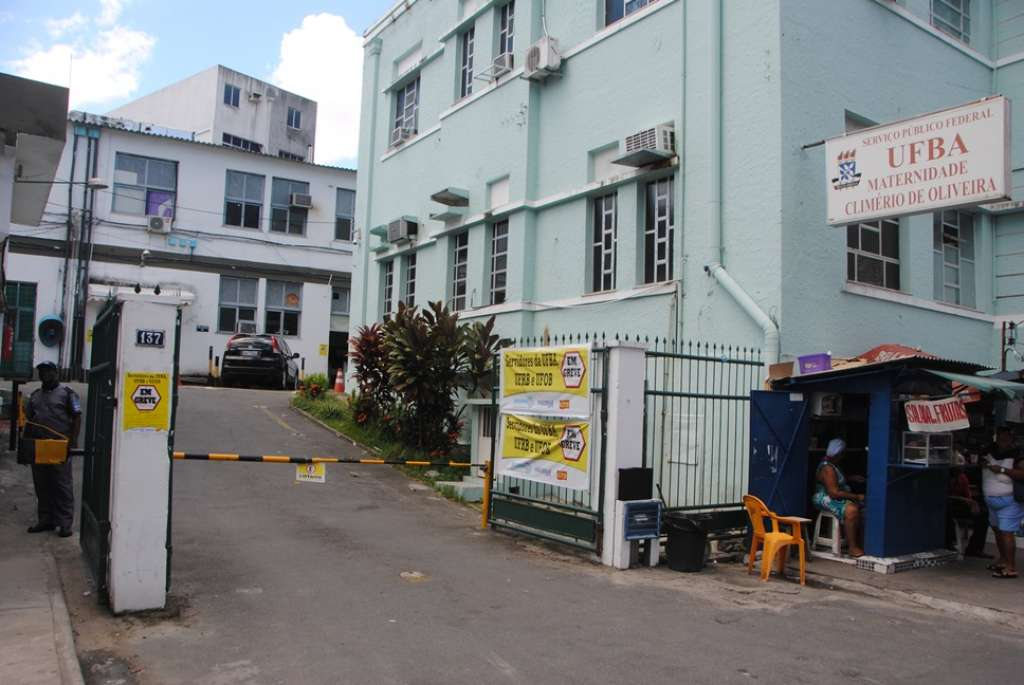
\includegraphics[width=0.39\textwidth]{maternidade}
    \end{wrapfigure}
    
    Hospital Maternidade de atendimento de emergência obstétrica 24 horas, acompanhamento pré-natal, ginecologista e Medicina Fetal

    
    \subsubsection{Dias da Semana e Horário de Funcionamento:}
            Emergência: 24 horas
    
    \subsubsection {Telefone de Atendimento ao Cidadão:}
            (71) 3283-9200

    \subsubsection{Email de Atendimento ao Cidadão:}
            ouvidoria.mco@ufba.br
    
    \subsubsection{Sistema de Sugestões e Reclamações:}
            Email: ouvidoria.mco@ufba.br \\ Telefone: (71) 3283-9200

    \subsubsection{Endereço de Atendimento:}
            Rua do Limoeiro, 137, Nazaré, Salvador - BA \\ 40055-150

    \subsubsection{Requisitos, documentos e informações necessárias para acessar o serviço:}
             Documentos básicos, como documento de identificação original com foto, e cartão SUS  
    \subsection{FOUFBA}
    
    A Faculdade presta serviços de atenção á Saúde Bucal e atendimento odontológico
        
    \subsubsection{Dias e Horários de atendimento:}
    A definir por meio de marcação que pode ser feita por telefone ou via presencial.
    
    \subsubsection{Telefone de Atendimento ao Cidadão:}
         (71) 3283-8980
        
    \subsubsection{Email de Atendimento ao Cidadão:}
        odo@ufba.br
        
    \subsubsection{Sistema de Sugestões e Reclamações:}
        Email: ouvidoria@ufba.br \\ Telefone: (71) 3283-7044
        
    \subsubsection{Endereço de Atendimento:}
         Avenida Araújo Pinho, 62 - Canela, Salvador - BA, 40110-040
         
    \subsubsection{Requisitos, documentos e informações necessárias para acessar o serviço:}
        Basta ser brasileiro (a) ou estrangeiro residente no Brasil e apresentar o Cartão Nacional de Saúde (CNS) ou Cartão SUS. 

    
